\documentclass[UTF8,a4paper,zihao=-4]{ctexart}
\usepackage[left=3.175cm,right=3.175cm,top=2.54cm,bottom=2.54cm]{geometry}
\usepackage{amsmath,amssymb,graphicx,booktabs,tabularx,array,setspace,caption,float}
\usepackage[unicode,hidelinks]{hyperref}
\usepackage{url}
\usepackage{newtxtext,newtxmath}
\usepackage{cite}
\onehalfspacing
\setlength{\parindent}{2em}
\setcounter{tocdepth}{2}
\ctexset{section={format=\heiti\zihao{-2}},subsection={format=\heiti\zihao{4}},subsubsection={format=\heiti\bfseries\zihao{-4}}}
\captionsetup{font=small,labelfont=bf}
\begin{document}
\begin{titlepage}
\centering
\vspace*{2.5cm}
{\heiti\zihao{2}北京上方山文物古迹的\\[0.3em]多源数据组织与数字化展示研究\par}
\vspace{2cm}
{\zihao{-3}
专业\quad 地理信息科学\\[0.8em]
姓名\quad \underline{\hspace{4cm}}\\[0.8em]
学号\quad \underline{\hspace{4cm}}\\[0.8em]
指导教师\quad 艾刚\par}
\vspace{1cm}
组员：周以勒\quad 王子帅\quad 肖艺骏\quad 汪楚雄\quad 孙兆麟
\vfill
2026年9月\\中国\quad 北京
\end{titlepage}
\pagenumbering{Roman}
\begin{center}{\heiti\zihao{-2}摘\quad 要}\end{center}


针对北京上方山寺庵、碑刻与历史建筑资料分散，文献记载、空间坐标和三维展示之间缺少清晰关联的问题，本文围绕“山河入卷”项目，开展文献梳理、多源空间数据组织及数字化展示研究。以《上方山志》、碑刻资料与地方研究为历史信息来源，结合项目坐标记录、数字正射影像（DOM）、数字表面模型（DSM）、实景三维数据和网页原型，建立历史实体、空间位置与展示内容之间的关联框架。通过读取影像世界文件、投影文件及三维生产报告，确认 DOM 与 DSM 的像元大小均为 0.3 m，平面参考为 CGCS2000 三度带高斯—克吕格投影第 39 带（EPSG:4527），并核实 16 个实景三维生产瓦块。以永亨庵为案例，将可由史料支持的方位与院落信息，同尚需论证的建筑形制区分表达；对网页中的 Canvas 地图、碑刻资料卡及 Three.js 模型接口进行功能分析。结果表明，现有数据能够支撑上方山文物信息的空间组织和展示原型，但部分点位的观测质量、模型的历史依据及网页资源完整性仍需补充验证。研究说明，多源资料整合的关键在于保持来源可追溯、坐标含义一致，并明确实景记录与推测性复原的边界。



\noindent\textbf{关键词：}上方山；文化遗产；多源空间数据；GNSS；GIS；数字化展示


\clearpage
\tableofcontents
\clearpage
\pagenumbering{arabic}


\section*{1 引言}
\addcontentsline{toc}{section}{1 引言}

\subsection*{1.1 问题的提出及研究意义}
\addcontentsline{toc}{subsection}{1.1 问题的提出及研究意义}

\subsubsection*{1.1.1 问题提出}
\addcontentsline{toc}{subsubsection}{1.1.1 问题提出}

上方山文物古迹依托山地环境分布，寺庵、碑刻、塔院与洞窟共同构成具有历史联系的文化景观。清代《上方山志》按山峰、寺庵等对象记录山中名胜，为认识其空间格局提供了文献线索\cite{r1}。《上方山访碑录》则为专题碑刻资料的查考提供了书目基础\cite{r2}。然而，古籍中的名称与现代地名并不总能直接对应，同一地点可能存在异名，现存碑石位置也未必等于历史建筑原址。将这些材料直接转写为地图上的确定点位，容易掩盖考证过程中的不确定性。


数字化展示还面临另一类问题：不同数据产品的功能和尺度差异较大。DOM 便于识别地物纹理，DSM 表达表面起伏，实景三维模型记录地物的几何与纹理，历史建筑示意模型则包含解释和推演。网页可以将它们置于同一界面，但界面上的关联不等同于空间配准，更不等同于历史复原得到验证。因此，本文关注如何在多源资料之间建立可检查的联系，使数字化成果既能用于阅读和展示，也能为后续测绘与研究保留依据。


\subsubsection*{1.1.2 研究意义}
\addcontentsline{toc}{subsubsection}{1.1.2 研究意义}

从遗产研究角度看，将历史对象与空间位置关联，有助于从孤立碑文扩展到寺庵、道路、山势及营建活动之间的联系。从地理信息实践角度看，对坐标参考、影像分辨率和模型原点进行统一说明，可以减少同名异物、坐标误置和模型错配。从公共展示角度看，以空间查询连接历史叙事，有助于读者理解文物所处的环境，而不仅是浏览若干文字和图片。


本文的工作重点是整理已有成果并建立可追溯的展示组织方法。对于缺少原始观测或直接形制证据的内容，保留其作为待研究对象的价值，同时避免把推测写成测量结果或考古结论。


\subsection*{1.2 相关工作与研究定位}
\addcontentsline{toc}{subsection}{1.2 相关工作与研究定位}

上方山历史研究中，古籍记载、碑刻录文和地方调查相互补充。杨亦武对上方山寺庵的介绍提供了永亨庵、福德庵、地藏殿等对象的方位和建筑遗存线索\cite{r3}；其有关上方山历史的文章讨论了明代寺院营建与奉藏佛经等活动\cite{r4}。这些资料的价值主要在于提出历史解释和空间约束，使用时仍须区分文献所描述的时代、后人调查所见状态以及现代网页的改写文字。


数字遗产研究强调展示过程的透明度。《伦敦宪章》要求说明可视化对象究竟属于现状记录、基于证据的复原还是假设性重建，并保存相关来源与推理过程\cite{r5}。这一原则尤其适用于建筑本体不存的遗迹：模型外观可以完整，但外观的完整不能替代证据的完整。空间数据方面，GeoTIFF 标准将栅格与地理参考信息相联系，为保存影像的坐标含义提供规范基础\cite{r6}。


本文以项目资料为基础，围绕历史信息整理、空间基准核验与网页展示组织展开研究。研究不开展插值方法优劣比较，也不将展示点位的分布直接解释为统计显著的遗产聚集格局。空间统计分析需要可靠的观测对象、抽样设计和误差说明，现阶段首先解决这些分析的资料前提。


\section*{2 研究区与数据来源}
\addcontentsline{toc}{section}{2 研究区与数据来源}

\subsection*{2.1 研究对象与资料范围}
\addcontentsline{toc}{subsection}{2.1 研究对象与资料范围}

研究以北京市房山区上方山的寺庵与碑刻为主要对象，围绕兜率寺及相关寺庵、古道和洞窟组织空间信息。地方研究所记录的永亨庵及其相邻寺庵，为讨论历史方位转化为地图位置提供了具体案例\cite{r3}。本文将研究对象分为寺庵等历史实体、碑文等文本对象和影像模型等数字资产；三类对象通过标识关联，避免用一张点位表混合表示所有内容。


资料范围包括项目坐标记录、2026 年 9 月的项目汇报 PPT、HTML 展示文件，以及项目资料集中的 DOM、DSM、OSGB/OBJ 模型与生产报告。资料集还包括移动端选点截图、ArcMap 点位标记截图和“选点.mxd”工程文件。影像和实景三维数据属于本研究使用的既有数据成果，本文不将其生产过程表述为研究团队本次新完成的航摄或扫描作业。


\subsection*{2.2 多源数据及用途}
\addcontentsline{toc}{subsection}{2.2 多源数据及用途}

数据按历史信息、空间记录、栅格产品、三维资产与展示材料组织，主要来源和使用边界见表 1。原始资料与展示用派生文件分别保存，研究中对影像采用降采样预览制图，不改变原始 GeoTIFF 及其配套文件。


\begin{table}[H]\centering\caption*{表 1 研究数据来源及用途}\small

\begin{tabularx}{\textwidth}{>{\raggedright\arraybackslash}X>{\raggedright\arraybackslash}X>{\raggedright\arraybackslash}X}\toprule

数据类型 & 资料内容 & 用途及边界 \\

\midrule

历史资料 & 《上方山志》、碑刻资料及地方研究 & 提取名称、沿革和方位；逐条区分原文与转述 \\

坐标与选点资料 & 项目坐标表、两张选点截图、MXD 工程 & 检查位置关系；不据截图认定观测精度 \\

DOM 与 DSM & 两幅 GeoTIFF 及 PRJ、TFW、辅助元数据 & 地物辨识、表面起伏表达与空间参考核验 \\

实景三维资产 & OSGB、OBJ、纹理、metadata.xml、product.json & 核验模型参考系、瓦块及生产记录 \\

展示材料 & 项目 PPT 与 index2(3).html & 分析叙事组织、界面功能和资源依赖 \\

\bottomrule\end{tabularx}\end{table}

\subsection*{2.3 影像分辨率与空间参考}
\addcontentsline{toc}{subsection}{2.3 影像分辨率与空间参考}

DOM 与 DSM 的列数均为 29 655，行数均为 30 638。DOM 为三波段 8 位影像，DSM 为单波段 32 位浮点栅格。两者世界文件给出的横向像元大小为 0.3 m，纵向像元大小为 −0.3 m，旋转项为零，左上角像元中心坐标一致。由此可以确认它们具有一致的标称格网参数；这一结果说明格网可对应，并不代替同名地物的独立配准精度检查。


图 2.1 展示两幅数据的降采样预览。DOM 提供山地植被、道路和建设用地等纹理信息；DSM 用连续色带表达表面高程。DSM 包含植被和建筑物等表面要素的影响，不能仅凭文件夹名称中的“DEM”将其当作经过地面点滤波的裸地数字高程模型。0.3 m 是像元大小，不是高程误差或定位误差。


\begin{figure}[H]\centering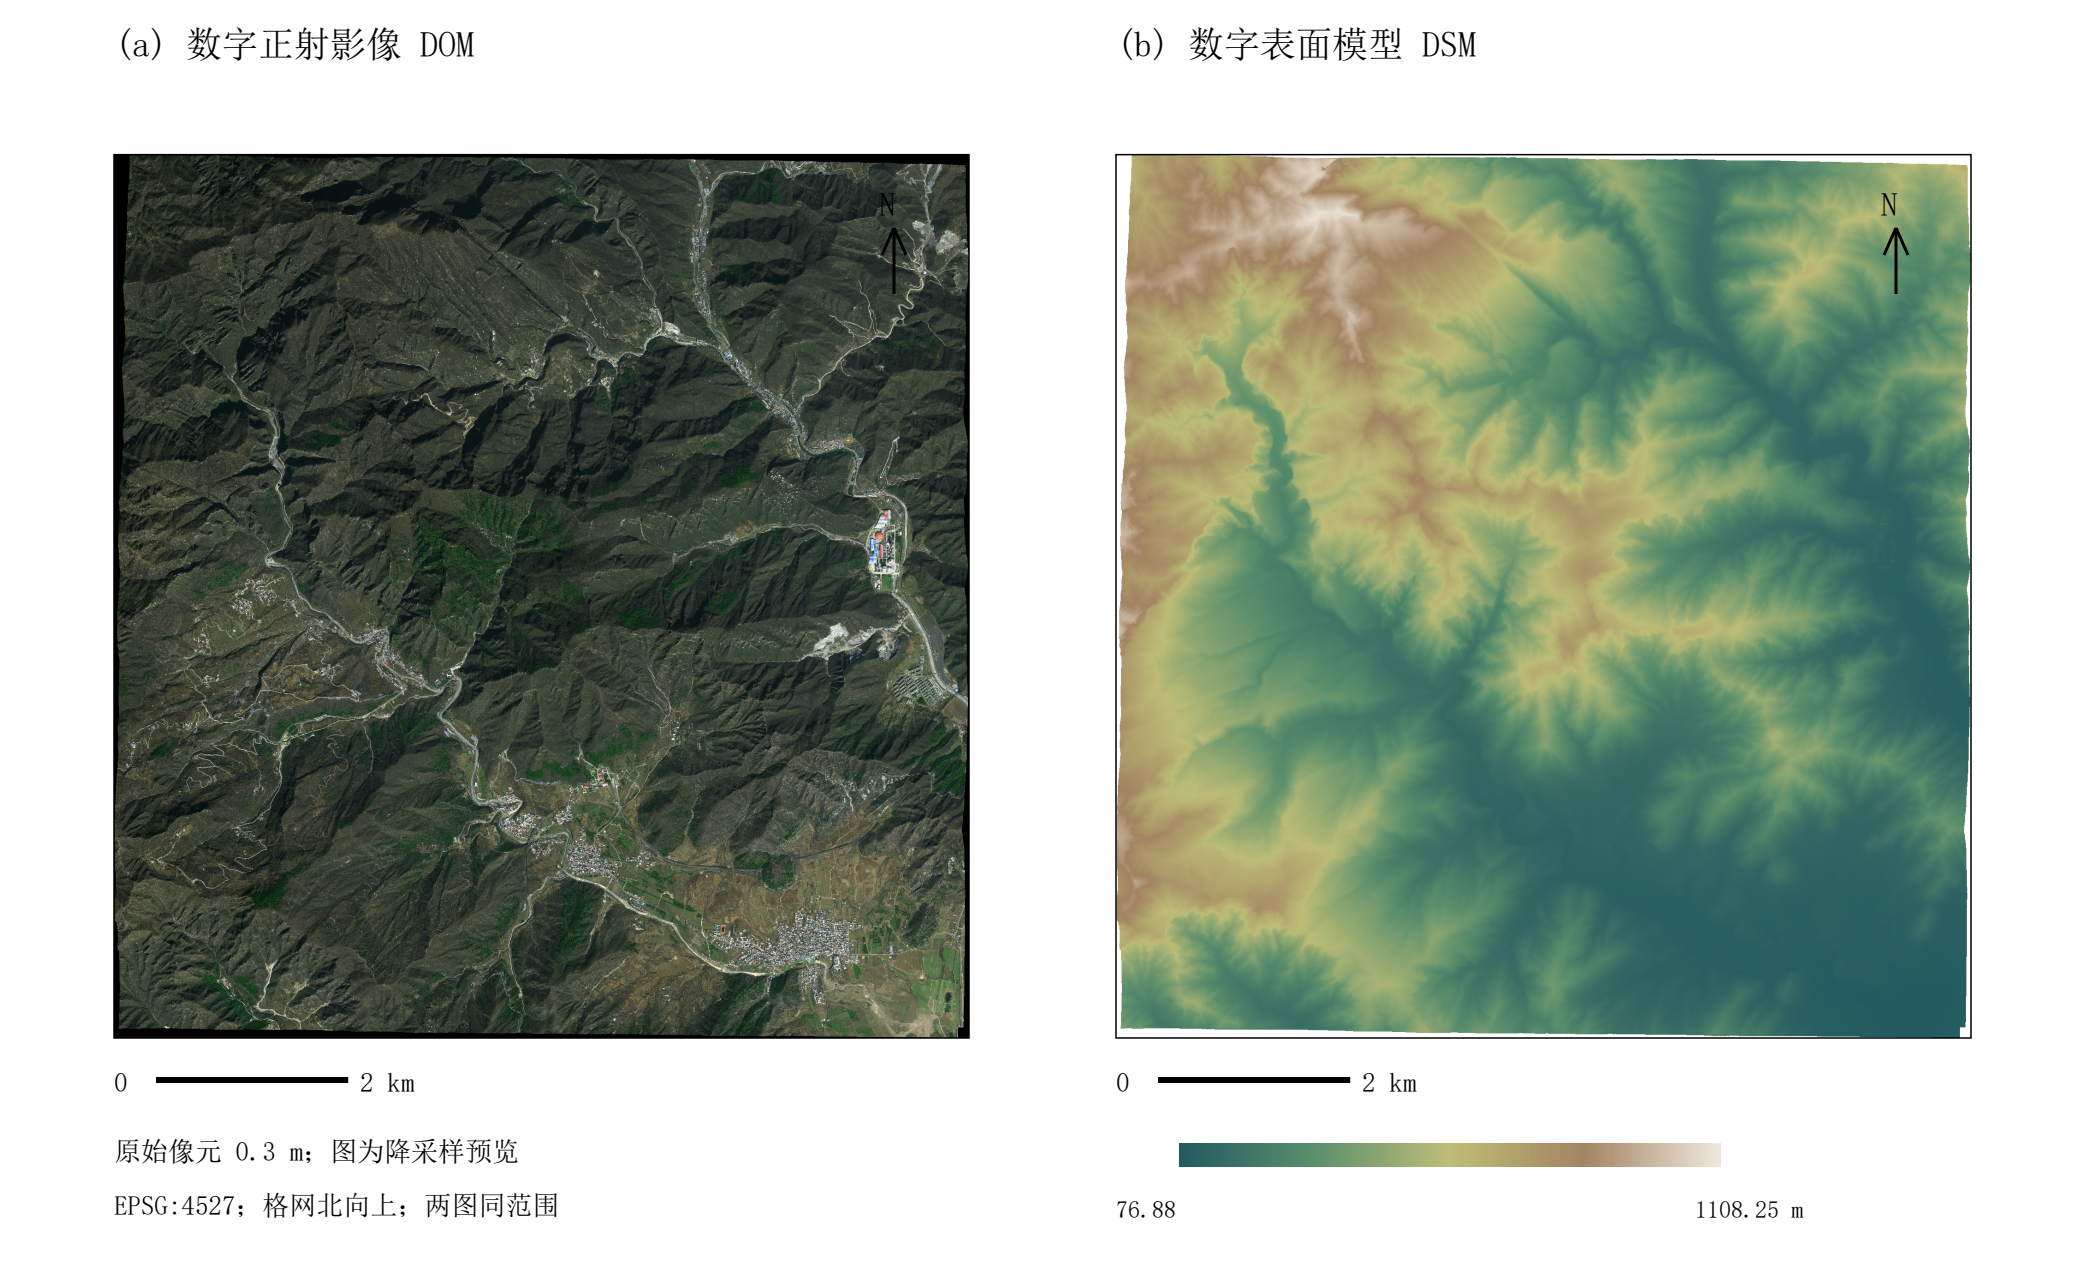
\includegraphics[width=\linewidth]{figures/imagery.png}\caption*{图 2.1 上方山 DOM 与 DSM 数据预览}{\footnotesize 来源：项目 GeoTIFF 数据及其已有概览层；DSM 色带按辅助元数据记录的最小值和最大值设置。\par}\end{figure}

两幅数据的 PRJ 文件均声明 EPSG:4527。该代码对应 CGCS2000 三度带高斯—克吕格投影第 39 带，中央经线为 117\textdegree{}E，假东移为 39 500 000 m\cite{r7}。这与模型 metadata.xml 的 SRS 字段一致。坐标轴含义必须按文件实际约定说明：本文用 E 表示东向坐标、N 表示北向坐标，避免软件中 X、Y 字段名称与测量学记号混淆。


\subsection*{2.4 数据质量与来源分级}
\addcontentsline{toc}{subsection}{2.4 数据质量与来源分级}

本文从来源、几何定位和展示三个层面记录资料状态。具有明确坐标参考和文件元数据的产品，可以用于空间组织；仅有项目说明而缺少原始观测记录的坐标，保留为项目记录，尚不能赋予确定的精度等级；文献给出的相对方位则作为位置判读的约束条件。对未定位对象，不以任意默认坐标代替缺失值。


项目记录载有 2026 年 9 月 1 日的手簿采点活动，但现有资料未形成包括仪器型号、观测时长、解状态、基站信息、点号对应关系与独立检核在内的完整记录。因此，本文保留 GNSS 在项目中的数据采集角色，不据此写出厘米级或毫米级的精度结论。项目 PPT 的成果数量与网页数据结构也采用各自统计口径，核对后再讨论其关系。


\section*{3 研究方法}
\addcontentsline{toc}{section}{3 研究方法}

\subsection*{3.1 总体技术路线}
\addcontentsline{toc}{subsection}{3.1 总体技术路线}

研究按“历史信息整理—空间数据核验—实体关联—数字展示”组织。先从志书及研究资料中提取对象名称、历史关系与方位，再对坐标记录、栅格和模型核查参考系与用途，随后建立历史对象与数字资产之间的关联，最后分析网页如何向读者呈现这些内容。图 3.1 列出各环节的主要输入与输出。


\begin{figure}[H]\centering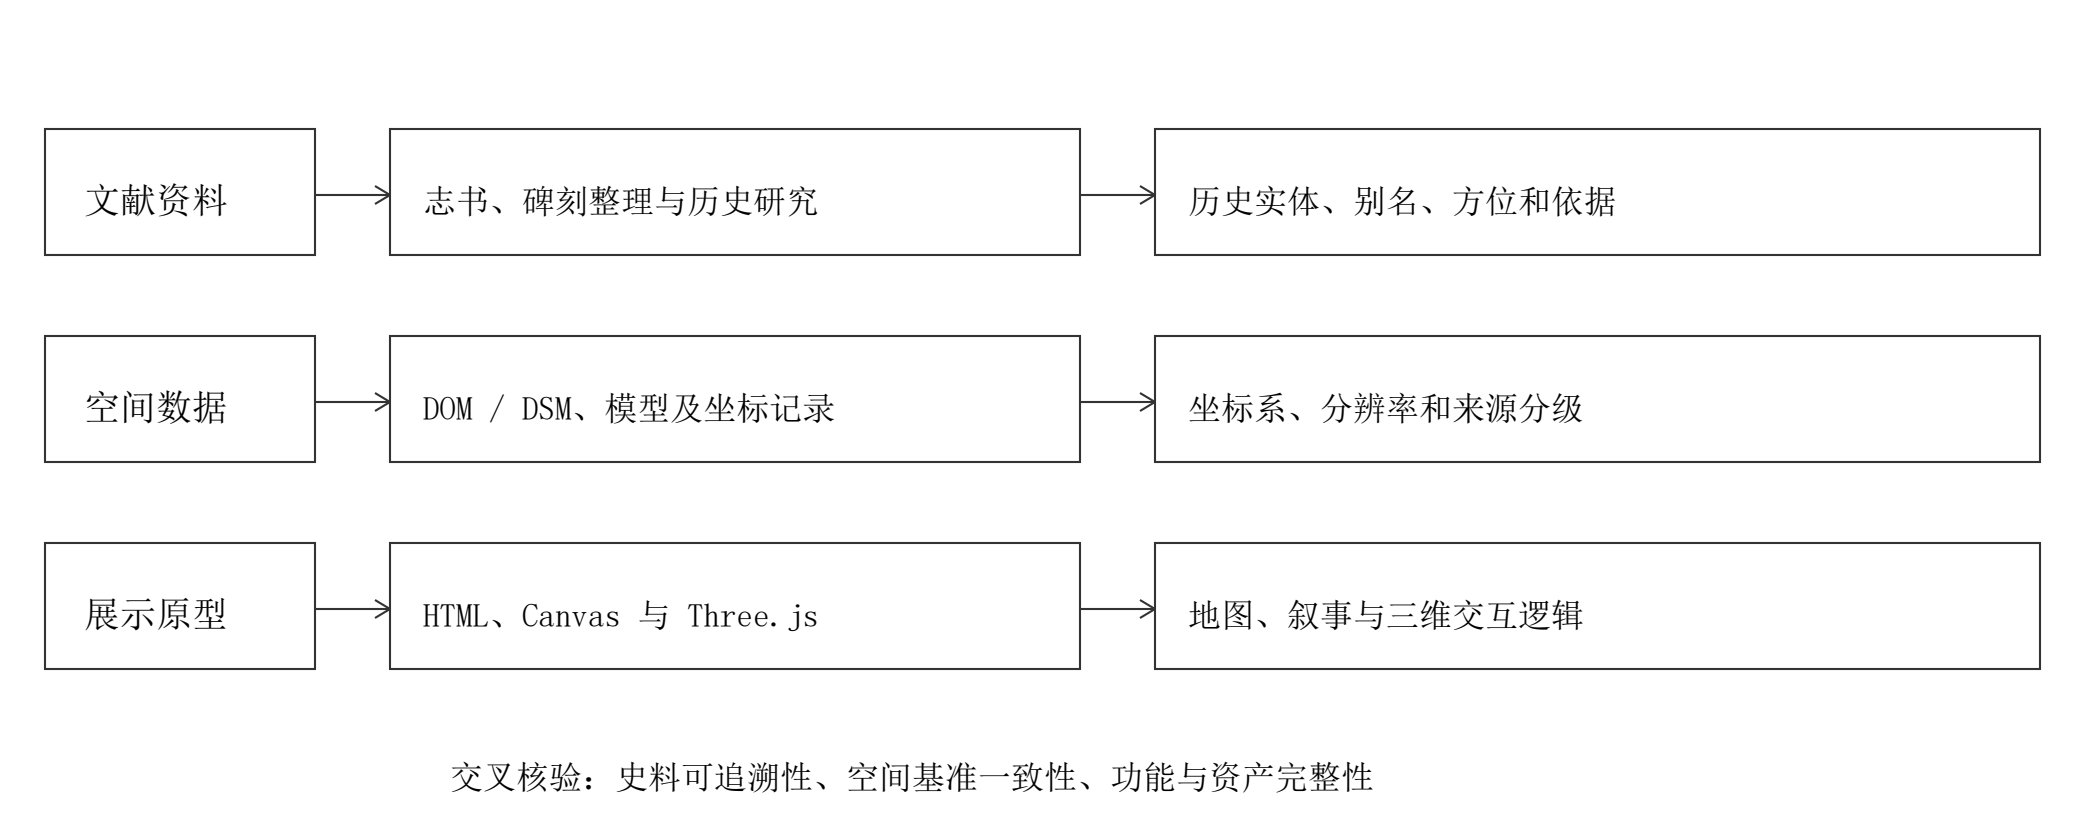
\includegraphics[width=\linewidth]{figures/workflow.png}\caption*{图 3.1 多源资料组织与数字化展示技术路线}{\footnotesize 来源：依据本研究资料组织流程绘制。\par}\end{figure}

文献信息与空间数据之间采用双向校验。文献说明某建筑位于另一建筑以西时，地图位置应当能够解释这一关系；空间位置不一致时，先检查同名异物、采点对象和坐标来源，再讨论历史地名变迁，不能只通过移动图标使其视觉上符合预期。模型与地图同样需要坐标对应和尺度检查，而非仅在页面中相邻摆放。


\subsection*{3.2 文献整理与历史实体关联}
\addcontentsline{toc}{subsection}{3.2 文献整理与历史实体关联}

文献整理以条目为单位，分别记录出处、对象、时代、空间关系与解释。原文摘录保留其出处；白话说明标记为转述；根据多条资料形成的判断标记为研究解释。对于电子古籍中的异体字、断句和疑似识读问题，保留原始记录并设置校核状态，不凭语感补字后再称为古籍原文。


历史名称与空间实体之间采用多对一或待定关系。永亨庵与永慈寺的名称关系需要结合沿革资料核对；“永慈庵”等相近名称不能仅因文字相似就自动合并。碑文、碑石与碑石所在寺庵也分别设置标识，一座寺庵可以关联多通碑石，一通碑石可以对应多个录文片段，计数时不将它们视为同一对象。


\begin{table}[H]\centering\caption*{表 2 历史实体与空间信息的建议关联字段}\small

\begin{tabularx}{\textwidth}{>{\raggedright\arraybackslash}X>{\raggedright\arraybackslash}X>{\raggedright\arraybackslash}X}\toprule

字段组 & 核心字段 & 作用 \\

\midrule

实体识别 & 实体编号、标准名称、历史别名、对象类型 & 区分实体、文本与别名 \\

历史依据 & 文献编号、条目定位、时代、原文或转述 & 保留信息出处及解释层级 \\

位置说明 & 坐标、参考系、定位方法、观测时间 & 区分观测点、推定位置和展示锚点 \\

质量状态 & 检核状态、误差指标、争议说明 & 防止未知精度被默认为高精度 \\

数字资产 & 图片路径、模型路径、模型类型、版本 & 连接地物、文献和展示内容 \\

\bottomrule\end{tabularx}\end{table}

\subsection*{3.3 栅格空间参考与坐标检查}
\addcontentsline{toc}{subsection}{3.3 栅格空间参考与坐标检查}

依据世界文件建立像元索引到投影坐标的对应关系。以左上角像元为第 0 行、第 0 列，列索引为 j，行索引为 i，本研究两幅栅格的像元中心坐标满足式（3.1）和式（3.2）。坐标单位为米。


\begin{equation}E(j)=39394844.0574946+0.3j\tag{3.1}\end{equation}

\begin{equation}N(i)=4398213.7456444-0.3i\tag{3.2}\end{equation}

世界文件记录的是像元中心，而地图范围通常采用像元外边界，计算范围时应在首末像元中心外侧加减半个像元。按行列数与像元大小计算，栅格矩形宽约 8.8965 km、高约 9.1914 km。这是数据外包矩形尺寸，不能直接视为文物保护范围或所有像元均有效的面积。


GNSS 经纬度、投影平面坐标与网页画布坐标分别管理。将 WGS84 坐标转换到 CGCS2000 相关成果时，需要明确参考框架、历元和项目精度需求，不能将二者差异固定写为某个毫米或厘米值。对项目资料提到的六组同名点仿射拟合，因缺少成对坐标、参数和残差记录，本文不将其作为已经完成精度检验的转换成果。


若后续使用独立检核点，可按式（3.3）计算平面位置均方根误差。式中，ΔE 与 ΔN 为成果坐标相对检核坐标的差值，n 为独立检核点数量。参与参数拟合的同名点残差只反映拟合情况，不能替代独立检核。本研究未获得满足条件的检核记录，因此不报告该指标的数值。


\begin{equation}\mathrm{RMSE}_{p}=\sqrt{\frac{1}{n}\sum_{i=1}^{n}(\Delta E_i^2+\Delta N_i^2)}\tag{3.3}\end{equation}

\subsection*{3.4 三维模型组织与复原依据}
\addcontentsline{toc}{subsection}{3.4 三维模型组织与复原依据}

三维资产分为实景三维成果和历史建筑示意模型。实景三维数据采用 OSGB 与 OBJ 两种形式，生产记录、空间参考及纹理是其组成部分。metadata.xml 提供 EPSG:4527 和局部原点，原点数值与 product.json 的对应字段相符。对于使用同轴、同单位局部顶点坐标的模型，可按原点平移关系恢复空间位置；具体导入软件仍须检查轴向和单位。


\begin{equation}E=E_0+x,\quad N=N_0+y,\quad Z=Z_0+z\tag{3.4}\end{equation}

其中，E₀ = 39 394 826.816825 m，N₀ = 4 389 128.530410 m，Z₀ = 64.707000 m。生产报告的高程字段标注为“正常高”，同时记录 EGM2008 改正文件。本文如实保留这一产品说明，不据此认定模型与特定国家高程基准已经完成水准联测。模型原点也不能直接移用于另一独立建模的建筑单体。


历史建筑示意模型需要另行说明依据。院落朝向和殿宇间数只能约束总体格局，不能直接确定钟楼的层数、屋顶形制、斗栱样式或构件尺寸。复原过程中应当把直接证据、同类建筑参照和展示性补足分别记录，并在模型说明中呈现不确定性\cite{r5}。因此，永慈寺钟楼在本文中定位为项目的建筑示意展示对象，不能等同于通过考古测绘验证的复原成果。


\subsection*{3.5 网页展示与交互组织}
\addcontentsline{toc}{subsection}{3.5 网页展示与交互组织}

HTML 原型包含叙卷、寺庙分布、石碑分布、七十二庵总览、文物、人物志、大事年表和摩崖石刻八个页面容器。叙卷将历史介绍、场景动画、碑刻阅读和钟楼展示串联；分布图提供空间入口，资料卡承担对象说明。该组织方式形成按故事阅读和按位置查询两种路径。


地图主体采用 Canvas 绘图，将经纬度在指定范围内线性映射到画布。代码使用的范围为东经 115.807\textdegree{}—115.828\textdegree{}、北纬 39.668\textdegree{}—39.679\textdegree{}，其对应关系见式（3.5）。其中 W、H 分别为画布宽高，u、v 为屏幕坐标，λ、φ 为经纬度。该转换用于绘制分布示意，不是高斯—克吕格投影转换，不能直接用于量算距离或面积。


\begin{equation}u=W\frac{\lambda-115.807}{0.021},\quad v=H\frac{39.679-\varphi}{0.011}\tag{3.5}\end{equation}

网页虽引用天地图 API，但已检查的地图绘制逻辑实际调用 Canvas，而未见利用天地图地图对象完成这两幅分布图的代码。底图由本地图片载入并拉伸至画布，代码未读取 GeoTIFF 的地理参考信息。因此，本文将其表述为轻量化分布展示，后续仍需核查底图裁剪范围、投影关系和地物配准。


钟楼部分使用 Three.js、GLTFLoader 和 OrbitControls。GLTFLoader 用于解析 glTF 资源，OrbitControls 提供围绕目标的视角控制\cite{r8,r9}。原型将载入模型按包围盒统一缩放、移至场景中心，并设置正视、侧视、俯视等视角。这种归一化服务于屏幕展示，不能据此读取建筑的真实尺寸。代码中未见结构拆解或线框切换的完整实现，不将其列为已验证功能。


\section*{4 结果与分析}
\addcontentsline{toc}{section}{4 结果与分析}

\subsection*{4.1 历史资料的空间关联}
\addcontentsline{toc}{subsection}{4.1 历史资料的空间关联}

永亨庵案例表明，文献中的邻接关系可以转化为空间核查条件。杨亦武的寺庵介绍将永亨庵置于福德庵以西，并描述其背南面北、两进院落的格局；地藏殿则位于永亨庵以西\cite{r3}。据此，可将永亨庵置于地藏殿以东作为相对方位约束，但不能仅由该关系推出精确坐标或完整建筑平面。


关于营建沿革，地方研究将冯保创建永亨庵和奉藏佛经联系于万历四年（1576）\cite{r4}。这一线索可以用于叙事组织和实体关联。对于藏经数量及其计量单位、敕名原文等更细的历史主张，应当回到具体碑文或可靠版本逐字校核；本文不以网页改写代替原典证据，也不把钟楼构件细节从寺院沿革中直接推导出来。


电子《上方山志》的“庵”条保存了寺庵名称序列，可作为名称整理的基础\cite{r1}。但网页动态经幡中的 45 个名称还包含泉、洞、殿和自然地貌等不同对象，因此它只能说明展示名称条目数，不能直接证明“45 所独立庵堂”的历史统计。异名、异体字及对象类型的统一，是进一步统计之前必须完成的工作。


\subsection*{4.2 栅格数据与实景三维成果}
\addcontentsline{toc}{subsection}{4.2 栅格数据与实景三维成果}

影像元数据和文件核验结果见表 3。两幅栅格具有相同的分辨率、行列数及定位参数，能够作为空间资料组织的共同底层。DSM 辅助元数据提供最小值、最大值、均值与标准差，可用于了解该产品记录的表面高程分布。以下统计为随附元数据值，未以本次独立外业重新验证；其中标准差描述表面高程离散程度，不是测量误差。


\begin{table}[H]\centering\caption*{表 3 DOM 与 DSM 的核实参数}\small

\begin{tabularx}{\textwidth}{>{\raggedright\arraybackslash}X>{\raggedright\arraybackslash}X>{\raggedright\arraybackslash}X}\toprule

指标 & DOM & DSM \\

\midrule

行列规模 & 29 655 列 \(\times\) 30 638 行 & 29 655 列 \(\times\) 30 638 行 \\

像元大小 & 0.3 m \(\times\) 0.3 m & 0.3 m \(\times\) 0.3 m \\

波段及类型 & RGB，8 位无符号整数 & 单波段，32 位浮点数 \\

平面参考 & EPSG:4527，第 39 带 & EPSG:4527，第 39 带 \\

NoData 标记 & TIFF 中未检出同类标记 & TIFF 标记值为 50 \\

表面高程最小值与最大值 & 不适用 & 76.88 m；1 108.25 m \\

表面高程均值与标准差 & 不适用 & 408.40 m；222.96 m \\

\bottomrule\end{tabularx}\end{table}

注：分辨率来自 TFW；坐标参考来自 PRJ 与 GeoTIFF；高程统计来自 DSM 的 AUX.XML。统计前应排除 NoData，不能将填充值 50 作为有效低程点。


三维生产报告记录了 16 个成功、0 个失败的逻辑瓦块，报告总耗时为 2 小时 20 分钟。文件清点得到 16 个 OBJ 文件和 1 945 个 OSGB 文件；前者与报告逻辑瓦块数量一致，后者包含分层或分块组织下的多个文件，不能把文件数当作独立测区数量。报告还记录 1 000 m 的分块长度参数、20 m 缓冲参数及 8 192 的最大纹理尺寸参数，这些属于生产配置，不能替代实景模型的几何精度指标。


\begin{figure}[H]\centering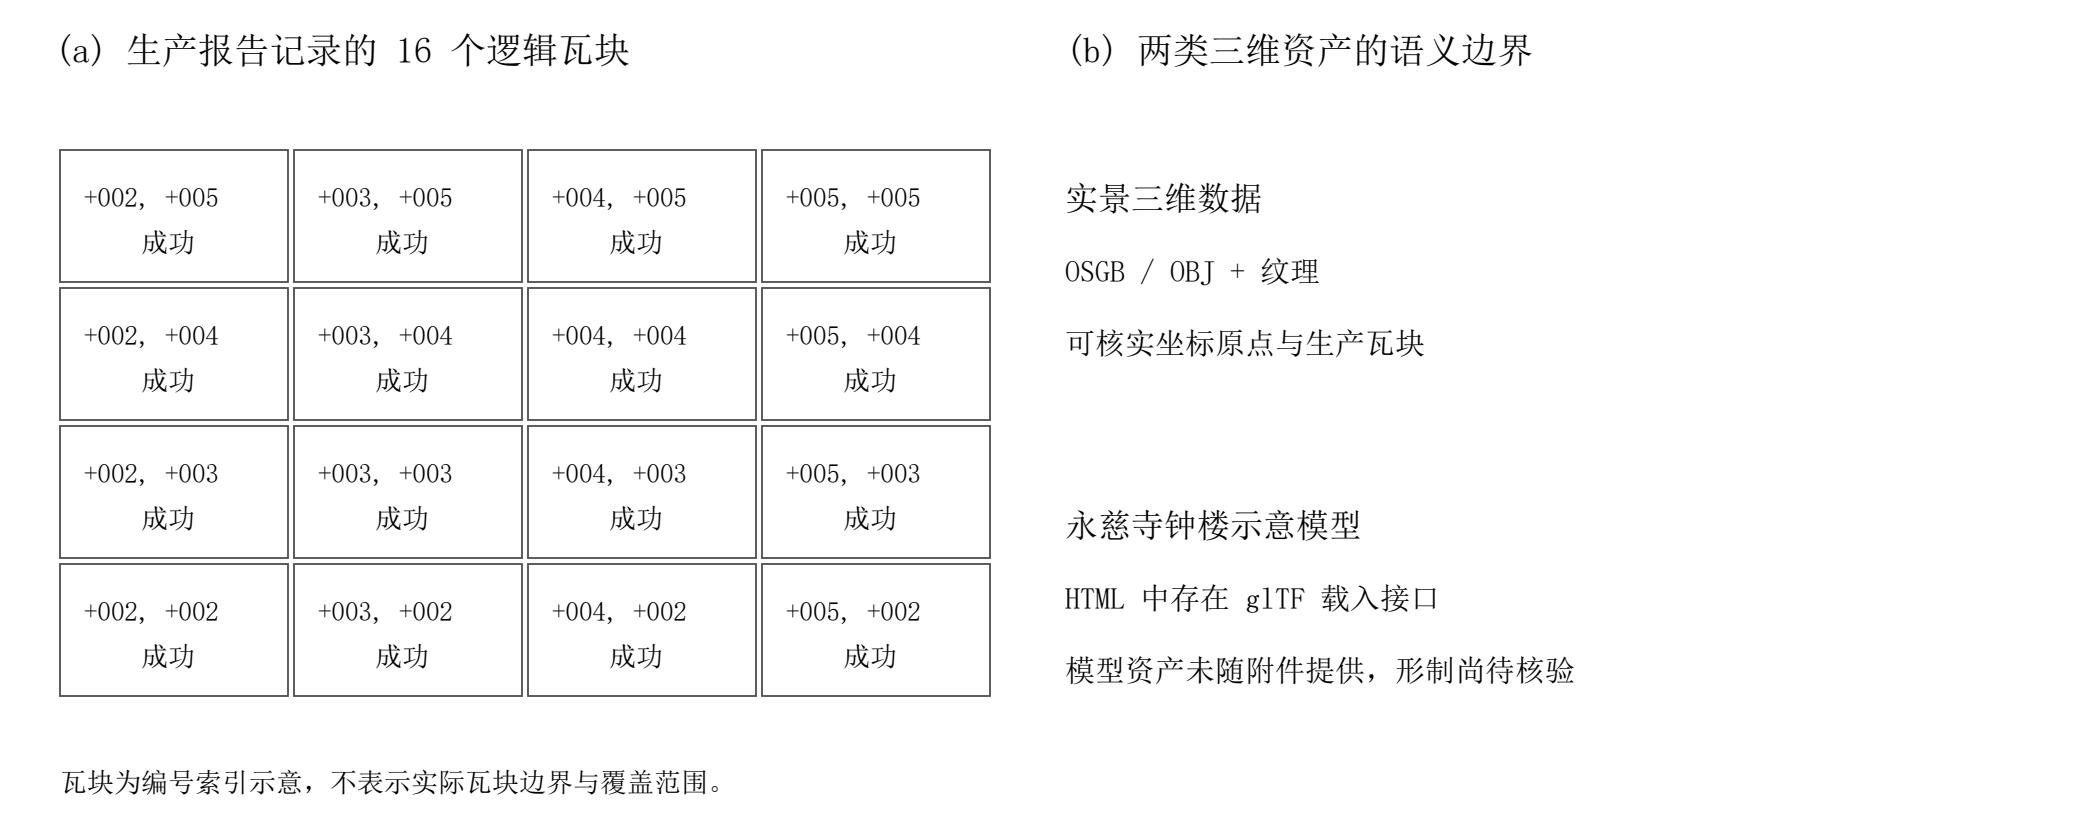
\includegraphics[width=\linewidth]{figures/tiles.png}\caption*{图 4.1 实景三维生产瓦块及模型类型区分}{\footnotesize 来源：项目 product.json、metadata.xml、模型文件清单及 HTML 代码。\par}\end{figure}

图 4.1 将生产瓦块与历史建筑示意模型区分。既有实景三维数据证明项目具有可供空间展示使用的模型资产；它不证明某个已经毁损的历史建筑得到精确复原。钟楼单体应有自己的模型文件、尺寸依据和版本说明，不能套用实景测区模型的坐标原点来宣称已完成地理配准。


\subsection*{4.3 坐标记录与选点资料核查}
\addcontentsline{toc}{subsection}{4.3 坐标记录与选点资料核查}

项目控制点表包含 10 个坐标记录，其经度约为 115.939\textdegree{}—115.954\textdegree{}；文物点位则主要分布在约 115.81\textdegree{}—115.82\textdegree{}附近。两组记录在空间上明显分离。以 G01 与兜率寺坐标计算，采用半径 6 371 km 的球面距离近似，直线距离约为 10.7 km。该计算仅用于识别资料范围差异，不作为测量精度评价。


两张项目图像分别展示移动端选点方案和 ArcMap 中的 10 个编号点（图 4.2）。它们能说明选点与地图标记的工作过程，但缺少点号对照及控制联测记录，不能据此证明控制点环绕上方山核心文物区，也不能证明控制网已直接约束这些文物点。本文据此将控制点记录保留为待核实的关联资料，不作“环状覆盖研究区”的结论。


\begin{figure}[H]\centering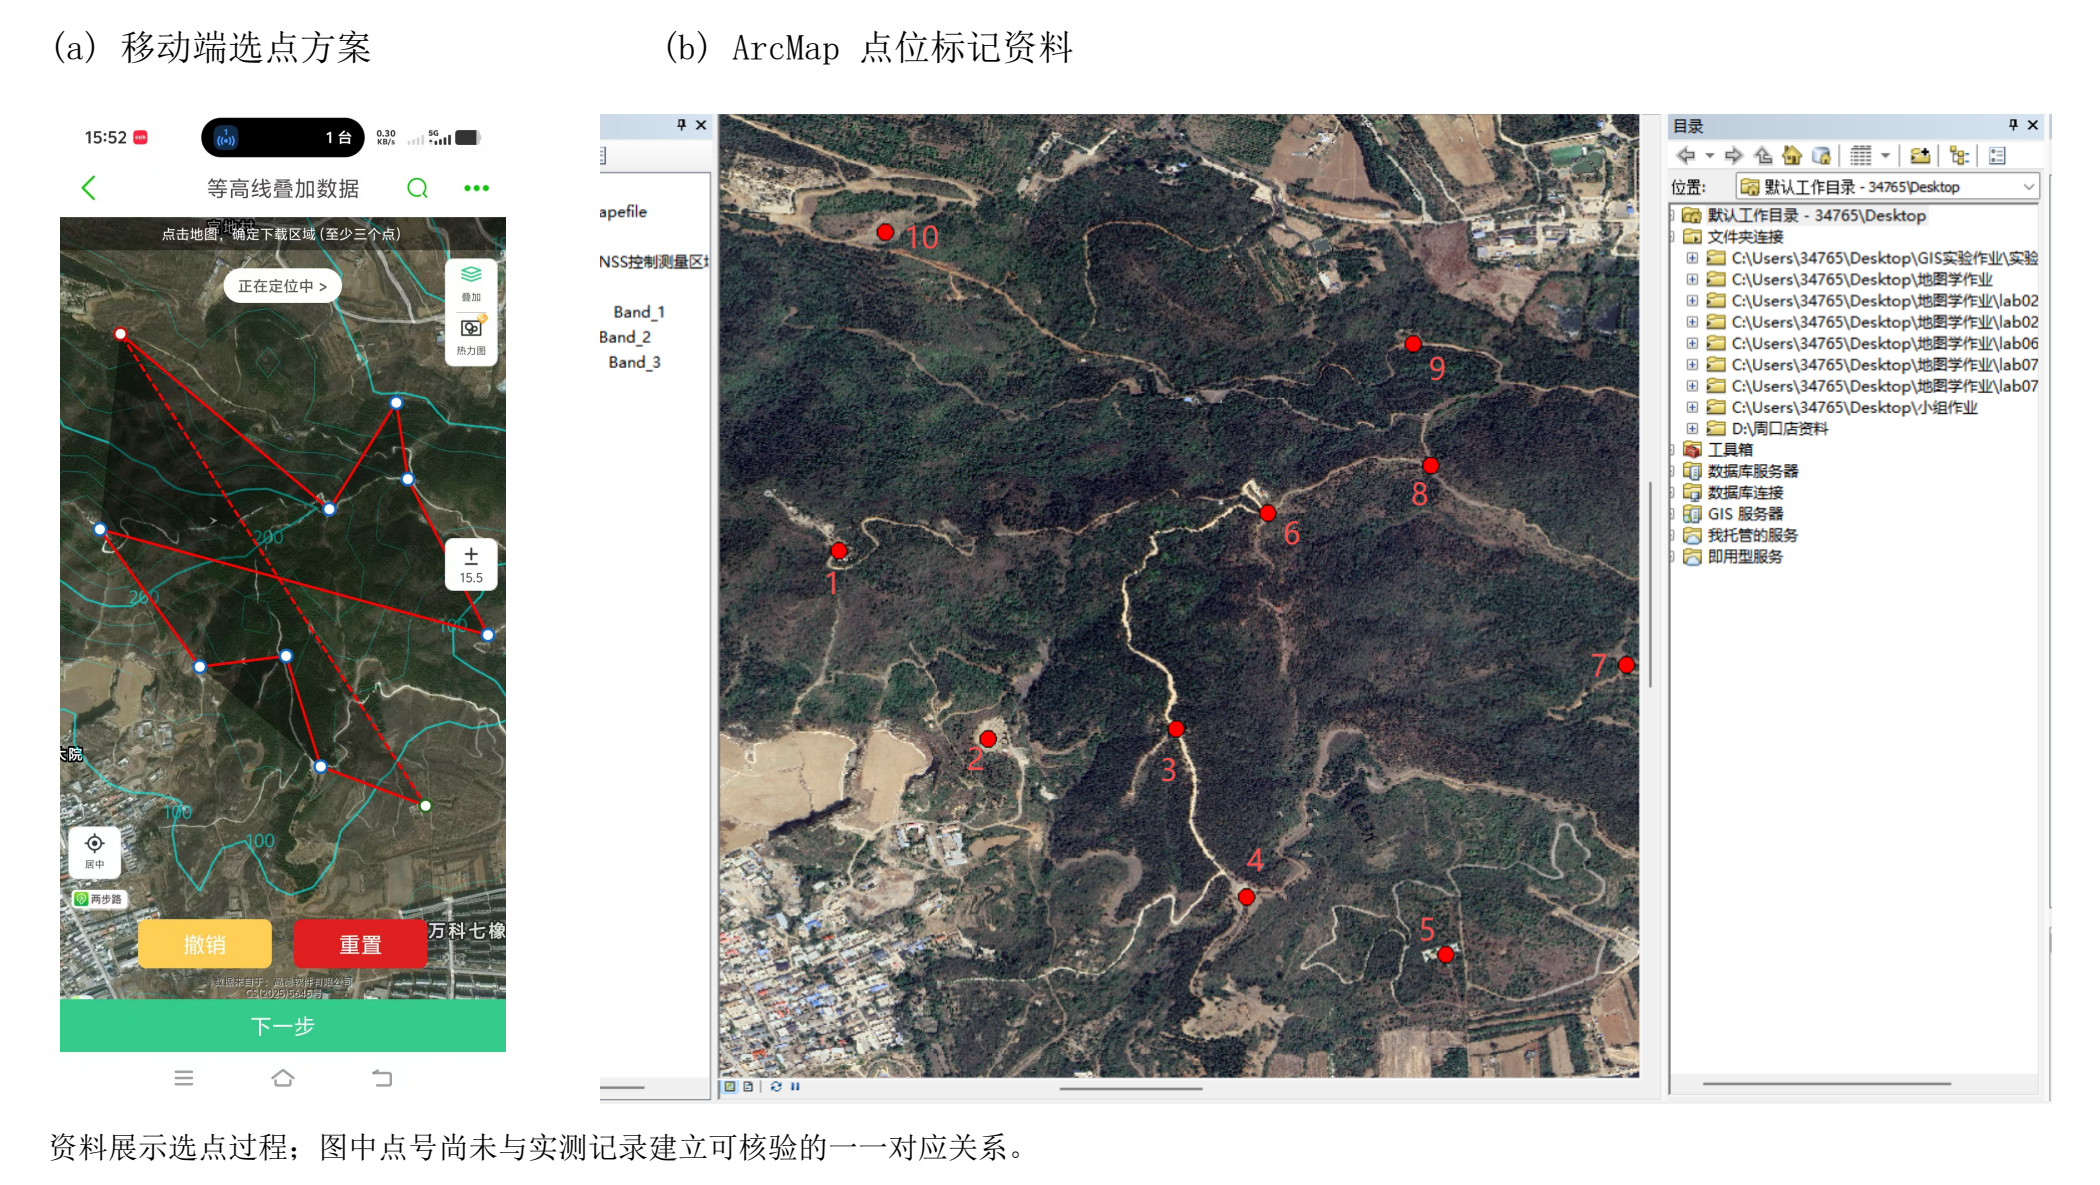
\includegraphics[width=\linewidth]{figures/selection.png}\caption*{图 4.2 移动端选点方案与 ArcMap 点位标记资料}{\footnotesize 来源：项目选点资料；保留原图信息，不将图中连线解释为已观测基线。\par}\end{figure}

\begin{table}[H]\centering\caption*{表 4 主要文物坐标记录与使用状态}\small

\begin{tabularx}{\textwidth}{>{\raggedright\arraybackslash}X>{\raggedright\arraybackslash}X>{\raggedright\arraybackslash}X>{\raggedright\arraybackslash}X}\toprule

对象 & 经度 E（\textdegree{}） & 纬度 N（\textdegree{}） & 项目所述来源与本文状态 \\

\midrule

兜率寺 & 115.822327 & 39.675888 & 手簿实测；待原始记录检核 \\

东门石碑 & 115.816666 & 39.663868 & 手簿实测；待原始记录检核 \\

云梯石碑群 & 115.822395 & 39.675873 & 手簿实测；需核对对象与点号 \\

永亨庵（永慈寺） & 115.822520 & 39.675300 & 仿射推算；参数与残差待补 \\

华严洞 & 115.822390 & 39.675740 & 仿射推算；参数与残差待补 \\

云水洞石刻 & 115.807490 & 39.666520 & POI 锚点；仅作参考位置 \\

\bottomrule\end{tabularx}\end{table}

注：表中数值来自项目坐标记录，不表示本研究重新采测；末位补零用于列对齐，不增加有效精度。项目将坐标标为 WGS84，其参考框架与观测历元尚需原始成果说明支持。


另一个值得核查的问题是对象识别。表 4 中兜率寺与“云梯石碑群”坐标仅相距约 6 m，与网页为天梯碑设置的展示位置并不一致。差异可能来自采点对象、分组方式或资料版本，不能只通过保留更多小数位解决。东门石碑和云水洞石刻的纬度均低于网页画布范围的南界 39.668\textdegree{}，若直接套用现有映射范围，将落在画布之外。因此，展示范围应依据经过核验的对象集合重新确定。


\subsection*{4.4 网页内容与功能边界}
\addcontentsline{toc}{subsection}{4.4 网页内容与功能边界}

网页代码形成了叙事页面与专题查询页面相结合的结构。寺庙分布图使用点选资料卡展示对象信息，石碑分布图设置碑文列表与跳转入口，钟楼场景提供模型载入和视角控制接口。碑林、诗文、人物志等内容由外部数据脚本驱动，体现出将内容与界面逻辑分开组织的意图。


HTML 原型引用了 7 个本地 JavaScript 数据文件，以及多张底图和背景图；其中包括碑文数据、寺庵数据和钟楼模型数据。现有资料中未见这些同名配套文件，实景三维模型也不能直接代替钟楼数据脚本。因此，可确认的是代码中的功能组织与调用逻辑，尚不能据单个 HTML 认定全部内容均可完整载入、无需网络运行或已通过跨设备测试。


\begin{table}[H]\centering\caption*{表 5 项目汇报与网页内容的统计口径}\small

\begin{tabularx}{\textwidth}{>{\raggedright\arraybackslash}X>{\raggedright\arraybackslash}X>{\raggedright\arraybackslash}X}\toprule

项目 & PPT 所述 & 当前材料能够核实的范围 \\

\midrule

GNSS 点位 & 37 处 & 缺完整原始点表，不能核实有效唯一点数 \\

可考碑文 & 38 篇 & HTML 设置 17 个碑题位置映射；全文依赖外部脚本 \\

庵堂名录 & 45 所 & 经幡代码含 45 个名称，但混有泉、洞及地貌等对象 \\

建筑模型 & 1 座 & 存在钟楼模型载入接口；单体数据未随附件提供 \\

\bottomrule\end{tabularx}\end{table}

“37 处点位”与“38 篇碑文”分别对应空间对象和文本对象，数值不同本身不构成错误，但需要关联表说明一处多碑或一碑多文的情况。石碑分布图代码中的 17 个题名也只是映射条目，不能直接替代已校勘碑文篇数。统计结果必须能回溯到具体记录，而不能只来源于汇报页面上的数字。


此外，网页为部分碑题使用所属寺庵的位置，未匹配题名采用共同默认位置。该逻辑便于展示，却会把“未知位置”变成看似确定的地图点，也可能造成多个对象人为聚集。后续应为坐标缺失对象设置“未定位”状态，仅在列表中展示其文献信息；近似位置则应注明定位依据，避免被当作精确导航点。


\section*{5 讨论}
\addcontentsline{toc}{section}{5 讨论}

\subsection*{5.1 多源信息整合的价值}
\addcontentsline{toc}{subsection}{5.1 多源信息整合的价值}

多源数据整合的价值在于使读者能够在不同证据之间转换视角。文献说明寺庵之间的历史关系，DOM 提供地物和道路背景，DSM 补充表面起伏，模型提供几何表达，网页提供访问入口。当每种材料的来源和用途被明确记录时，展示页面可以进一步成为资料发现与研究核查的入口。


本研究的核验同时说明，数据名称相似并不代表产品含义相同。DSM 与裸地 DEM 不同，实景三维与历史复原不同，模型坐标原点与建筑尺寸不同，地图上的显示点与经过质量控制的观测点也不同。这些区分决定了成果能够回答什么问题，是后续功能扩展和研究分析的基础。


\subsection*{5.2 空间精度与统计分析前提}
\addcontentsline{toc}{subsection}{5.2 空间精度与统计分析前提}

在现阶段，具有明确参数的影像与模型可以支撑定位检查和背景展示，但点位记录的来源一致性与观测质量仍需完善。将参考点与实测点混合后直接进行核密度分析、最近邻分析或空间插值，可能把人为布点、默认坐标及版本差异解释为真实空间规律。对历史遗产对象，还应考虑遗存存续、调查覆盖与文献保存的选择性，避免将“已收录对象”视为完整总体。


后续应优先补齐点号、对象照片、采集时间、坐标框架与质量指标，并使用独立检核点评价位置误差。如果研究进一步涉及坡度、视域或通行分析，还需依据任务选择适当的高程产品；直接使用含树冠与建筑的 DSM 时，应说明这些表面要素对结果的影响。本文不以未开展的分析填充结论。


\subsection*{5.3 复原透明度与展示表达}
\addcontentsline{toc}{subsection}{5.3 复原透明度与展示表达}

钟楼示意模型可以帮助读者理解建筑体量和交互展示方式，但历史真实性需要依靠具体证据讨论。依据《伦敦宪章》的原则，模型说明应能回答采用了哪些资料、哪些部分来自直接证据、哪些部分属于解释，以及证据变化时哪些构件需要调整\cite{r5}。这比仅以“高保真”描述模型更有助于后续研究。


网页中“志原文”标签下的现代说明文字亦需逐条核对。带有现代计量单位、现状评价或编者解释的段落，不宜未经校核就作为清代原文引用。展示层可分别呈现原典图像或录文、白话解释与考证说明，使易读性与可追溯性同时得到保留。


\subsection*{5.4 后续完善方向}
\addcontentsline{toc}{subsection}{5.4 后续完善方向}

后续工作首先是完成数据归档和关联：补齐 HTML 配套资源，为历史实体、碑刻文本和模型设置稳定标识，并明确文件版本。其次是开展空间检核：核对控制点所属测区、整理原始 GNSS 记录、验证影像和点位叠加关系。完成这些工作后，再增加搜索、导出和多端适配等服务功能，并通过实际用户任务测试评价其可用性。


三维方面，应先补充钟楼的模型文件与形制依据，分别验证几何尺度、坐标定位和历史解释，再讨论院落级场景。AR 导览、多语言与更复杂的空间分析可以作为拓展方向，但需要相应数据、设备和测试支持，不能仅凭界面构想写成既有成果。


\section*{6 结论}
\addcontentsline{toc}{section}{6 结论}

本文围绕北京上方山文物古迹数字化展示，结合历史资料、项目坐标记录、DOM/DSM、实景三维数据和 HTML 原型，完成多源资料组织与关键参数核验，得到以下结论。


（1）历史资料能够为寺庵名称、沿革和相对方位提供线索。以永亨庵为例，可将文献描述转化为空间核查条件，但现有依据不足以直接确定精确建筑平面和钟楼构件形制。原文、转述与研究解释需要分层保存。


（2）DOM 与 DSM 具有相同的 0.3 m 像元和格网定位参数，平面参考均为 EPSG:4527，即 CGCS2000 第 39 带、中央经线 117\textdegree{}E。实景三维生产报告及文件清单共同支持 16 个逻辑瓦块的记录，为空间背景表达和模型组织提供了可核实的数据基础。


（3）项目控制点与核心文物点位在空间上明显分离，现有选点截图不能证明二者已完成控制联测。点位应按来源和检核状态使用，不能将坐标小数位数、影像分辨率或产品参数当作测量精度。


（4）网页原型形成了叙事、分布图和三维展示接口相结合的内容结构。其地图采用 Canvas 线性映射，钟楼依赖外部模型资源；展示位置与模型归一化不能替代空间配准。补齐资源、统一统计口径和完善证据记录，是由展示原型走向可靠研究平台的前提。


\section*{7 学习感悟}
\addcontentsline{toc}{section}{7 学习感悟}

本次实践使我们认识到，地理信息技术的应用不仅是把文字放到地图上，还需要解释对象是什么、坐标从何而来，以及不同资料是否描述同一个地点。检查影像分辨率、投影带号和模型原点的过程，让我们对空间参考的实际意义有了更具体的理解；整理寺庵名称和碑文条目的过程，也使我们体会到历史材料与空间数据在表达方式上的差异。


项目还提醒我们，展示效果与研究结论应分别评价。流畅的页面和完整的三维外观可以改善阅读体验，但不能代替观测记录与文献依据。今后的实践中，我们将更加重视原始资料归档、数据质量说明和团队协作中的版本管理，使每一项成果都能被解释、检查和继续使用。


\clearpage\addcontentsline{toc}{section}{参考文献}\begin{thebibliography}{99}

\bibitem{r1}达闻. 上方山志·庵[EB/OL]. 吴仁敌, 较订. 识典古籍[2026-09-10]. \url{https://www.shidianguji.com/book/HY0318/chapter/1k29z3oguh1je}.

\bibitem{r2}上方山国家森林公园管理处. 上方山访碑录[M]. 北京: 学苑出版社, 2023.

\bibitem{r3}杨亦武. 上方山七十二庵[EB/OL]. 北京市房山区政协资料[2026-09-10]. \url{https://zx.bjfsh.gov.cn/docs/20180829181320073608.pdf}.

\bibitem{r4}杨亦武. 上方名山佛国净土[EB/OL]. 北京市房山区政协资料[2026-09-10]. \url{https://zx.bjfsh.gov.cn/docs/20180829180728808768.pdf}.

\bibitem{r5}The London Charter. The London Charter for the Computer-based Visualisation of Cultural Heritage: Version 2.1[EB/OL]. (2009-02-07)[2026-09-10]. \url{https://www.london-charter.org/media/files/london_charter_2_1_en.pdf}.

\bibitem{r6}Open Geospatial Consortium. OGC GeoTIFF Standard: Version 1.1, 19-008r4[S/OL]. 2019[2026-09-10]. \url{https://docs.ogc.org/is/19-008r4/19-008r4.html}.

\bibitem{r7}Open Geospatial Consortium. CGCS2000 / 3-degree Gauss-Kruger zone 39, EPSG:4527[EB/OL]. [2026-09-10]. \url{https://opengeospatial.github.io/ontology-crs/data/def/crs/EPSG/0/4527/index.html}.

\bibitem{r8}Three.js. GLTFLoader[EB/OL]. [2026-09-10]. \url{https://threejs.org/docs/pages/GLTFLoader.html}.

\bibitem{r9}Three.js. OrbitControls[EB/OL]. [2026-09-10]. \url{https://threejs.org/docs/pages/OrbitControls.html}.

\end{thebibliography}

\end{document}